\documentclass[final,10pt,times,twocolumn]{elsarticle}
\usepackage[top = 4cm, bottom = 3cm, right = 2cm, left = 2cm, a4paper]{geometry}
\usepackage{amssymb}
\usepackage[backref]{hyperref}
\usepackage{booktabs}
\usepackage[version=4]{mhchem}

\hypersetup{
    colorlinks=true,
    linkcolor=blue,
    filecolor=magenta,      
    urlcolor=cyan,
    pdftitle={Overleaf Example},
    pdfpagemode=FullScreen,
    }
\usepackage{color}
\author{Jhih-Jia Hung}

\begin{document}
\begin{frontmatter}
\title{Uranium diboride, the potential candidates of ATF, feature and application \\ \LaTeX}
\begin{abstract}
It is universally acknowledged that power generation is most fundamental facility required by every industry, as almost all things require electricity to work. Among all the methods of electricity generation, nuclear power always faces considerable scrutiny. Undoubtedly, nuclear power brings about feelings of fear and unknown horror, especially after the accidents at Fukushima and Chernobyl. Such concerns are not unreasonable, as people's fear of nuclear power is a good measure to prevent accidents from happening. However, Taiwan people are too afraid of using this technology, turns out the result is miss out the opportunity to improve our ecosystem and make it more environmentally friendly. In this research, I would put the focus on the potentially fuel, Uranium diboride \ce{UB2}, an interesting fuel that nowadays are research to be an ATF candidate fuel. Its physical properties also make it suitable for use in GEN-IV reactors, which require high standards to reaction. All of these factors make \ce{UB2} show on my eyes, and this research aims to explore its potential.
\end{abstract}

\begin{keyword}
ATF, Uranium diboride, GEN-IV
\end{keyword}

\end{frontmatter}

\section{Introduction}
Uranium diboride is potentially material which on closely debating to be the next generation reactors fuel, expecialy known as ATFs( Advanced Technology Fuels or Accident Tolerance Fuels ). \ce{UB2} have unique talent that play a important role in. And ATFs is aim to increase the reactors power up-rates, longer cycle lengths, improved performance,and reduced stored energy in the core etc. And allow have more time to coping during accident scenarios.\cite{watkins2022challenges}

\begin{figure}[ht]
    \centering
    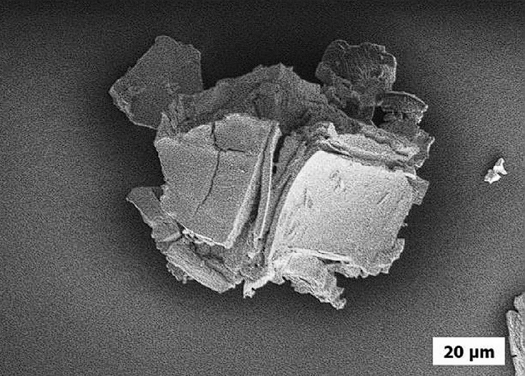
\includegraphics[width = 5.75cm]{UB2 Micrographs.png}
    \caption{UB2 Micrographs Picture\cite{watkins2022challenges} }
\end{figure}

\section{History}
The accident of Fukushima is the most impactable nuclear accident in 2011th, after Fukishima daiichi power plant accident, many country and organization going to figure out why the accident happened and find out solutions, althought theres a big part of research is about the Zircaloy Cladding technology, but it also gave rise to the development of a new field, ATF.

ATF has a lot of candidates, like \ce{U2Si3}, \ce{UC}, \ce{UN}, \ce{UB2} and some kind of material is on debating. Such that, the next-generation reactors(GEN-IV Reactor) has benefited on these development, with ATFs, the reactor can function more safety and efficiency.

\ce{UB2} has great talent to be the LWR(Light Water Reactors), PBR(Pebble Bed Reactors) and some kind of FBR reactors fertile fuel material.

\section{Properties}
In many candidate of ATFs material, the Uranium diboride has higher Uranium density than the others. Also, it has better thermal conductive that make itself have lower fuel centre-line temperatures on working, result in many positive effect such like; reduce the rate of temperature-dependent release of fission products, reduce the energy stored inside the fuel ( This properties also is the most important that the UB2 need. )

\subsection{Neutron Poison}
In last century, physicist found that there have a special material will absorb the thermal neutron in reactors, that is "Boron". 

\begin{table*}[ht]
    \centering
    \caption{The abundance and thermal neutron cross-section reaction type}
    \label{tab:my-table}
    \resizebox{\textwidth}{!}{%
    \begin{tabular}{llll}
    \hline
    Boron isotope (Mass Number) & Abundance(a/o)& The Cross-section of Thermal Neutron (Barn) & Reaction Type \\ \hline
    $B-9$  & trace                              &  -                                 & -                \\
    $B-10$ & 19.8\cite{JPCS_1696_1_012006bib1}  &  3837\cite{JPCS_1696_1_012006bib1} & Alpha Absorption \\
    -      &   -                                &  0.5                               & Gamma Absorption \\
    $B-11$ & 80.2\cite{JPCS_1696_1_012006bib1}  &  0.01                              & Gamma Absorption \\
    $B-12$ & trace                              &  -                                 & -                \\ \hline
    \end{tabular}%
    }
\end{table*}

Boron has two main isotope in the natural, Boron-10( B-10, natural abundance is $19.8\%$) and Boron-11 ( B-11, natural abundance is $80.2\%$ ), like Table 1. Boron-10's high cross-section make it will capture more thermal neutron then obstruct fissile fuel capture thermal neutron and finally stop the reaction after decay heat was cool down.

This properties make boron have a long time ago to be the material of neutron absorber in control rods, and nerver consider about to explored as fuel materials. But, after the accident of Fukushima daiichi, the Boron-10 begin to research on ATF.

Boron-10's high neutron cross-section makes it particularly effective at capturing thermal neutrons. This properties enable boron-10 to serve as a "Control Poison" within the broader category of "Neutron Poisons."\\

\begin{equation}
    ^{10}_{5}\ce{B} + ^{1}_{0}\ce{n} \rightarrow ^{7}_{3}\ce{Li} + \alpha    
\end{equation}

If boron-10 capture a thermal neutron like (1), it will release Lithum-7 and a alpha particle, this reaction is also been applied on BNCT( Boron Neutron Capture Treatment ).

Althought alpha particle( Helium-4 nuclei ) is ionization radiation and have very high ionization abillity, it can't release neutron and will slow down the reaction in reactor.\\

\begin{figure}[ht]
    \centering
    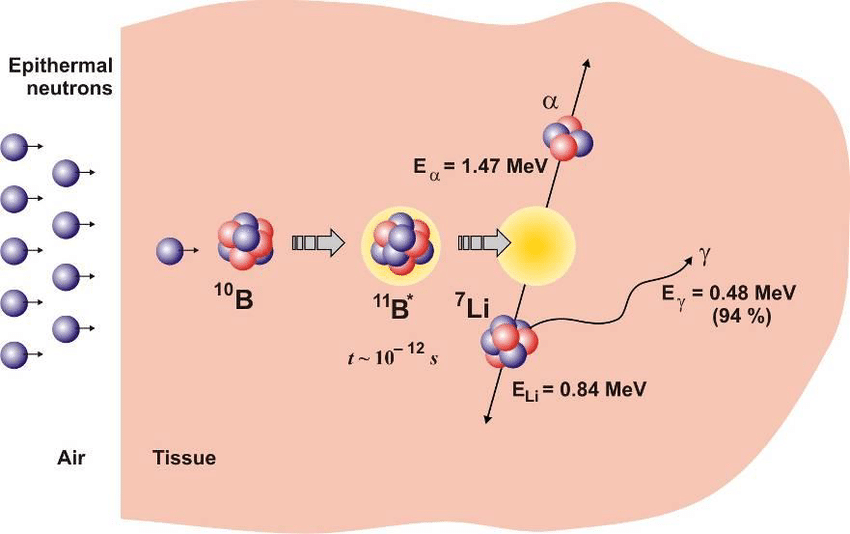
\includegraphics[width = 5.75cm]{BNCT.png}
    \caption{The Boron-10 in BNCT radiation reaction\cite{Kasatov_2016} }
\end{figure}

\begin{equation}
    ^{11}_{5}\ce{B} + ^{1}_{0}\ce{n} \rightarrow ^{12}_{4}\ce{B} + \gamma
\end{equation}

Boron-11 is not a good neutron absorption, if Boron capture thermal neutron, its mostly reaction chain is like (2) and still can not release neutron to keep chain-reaction.

\begin{figure}[ht]
    \centering
    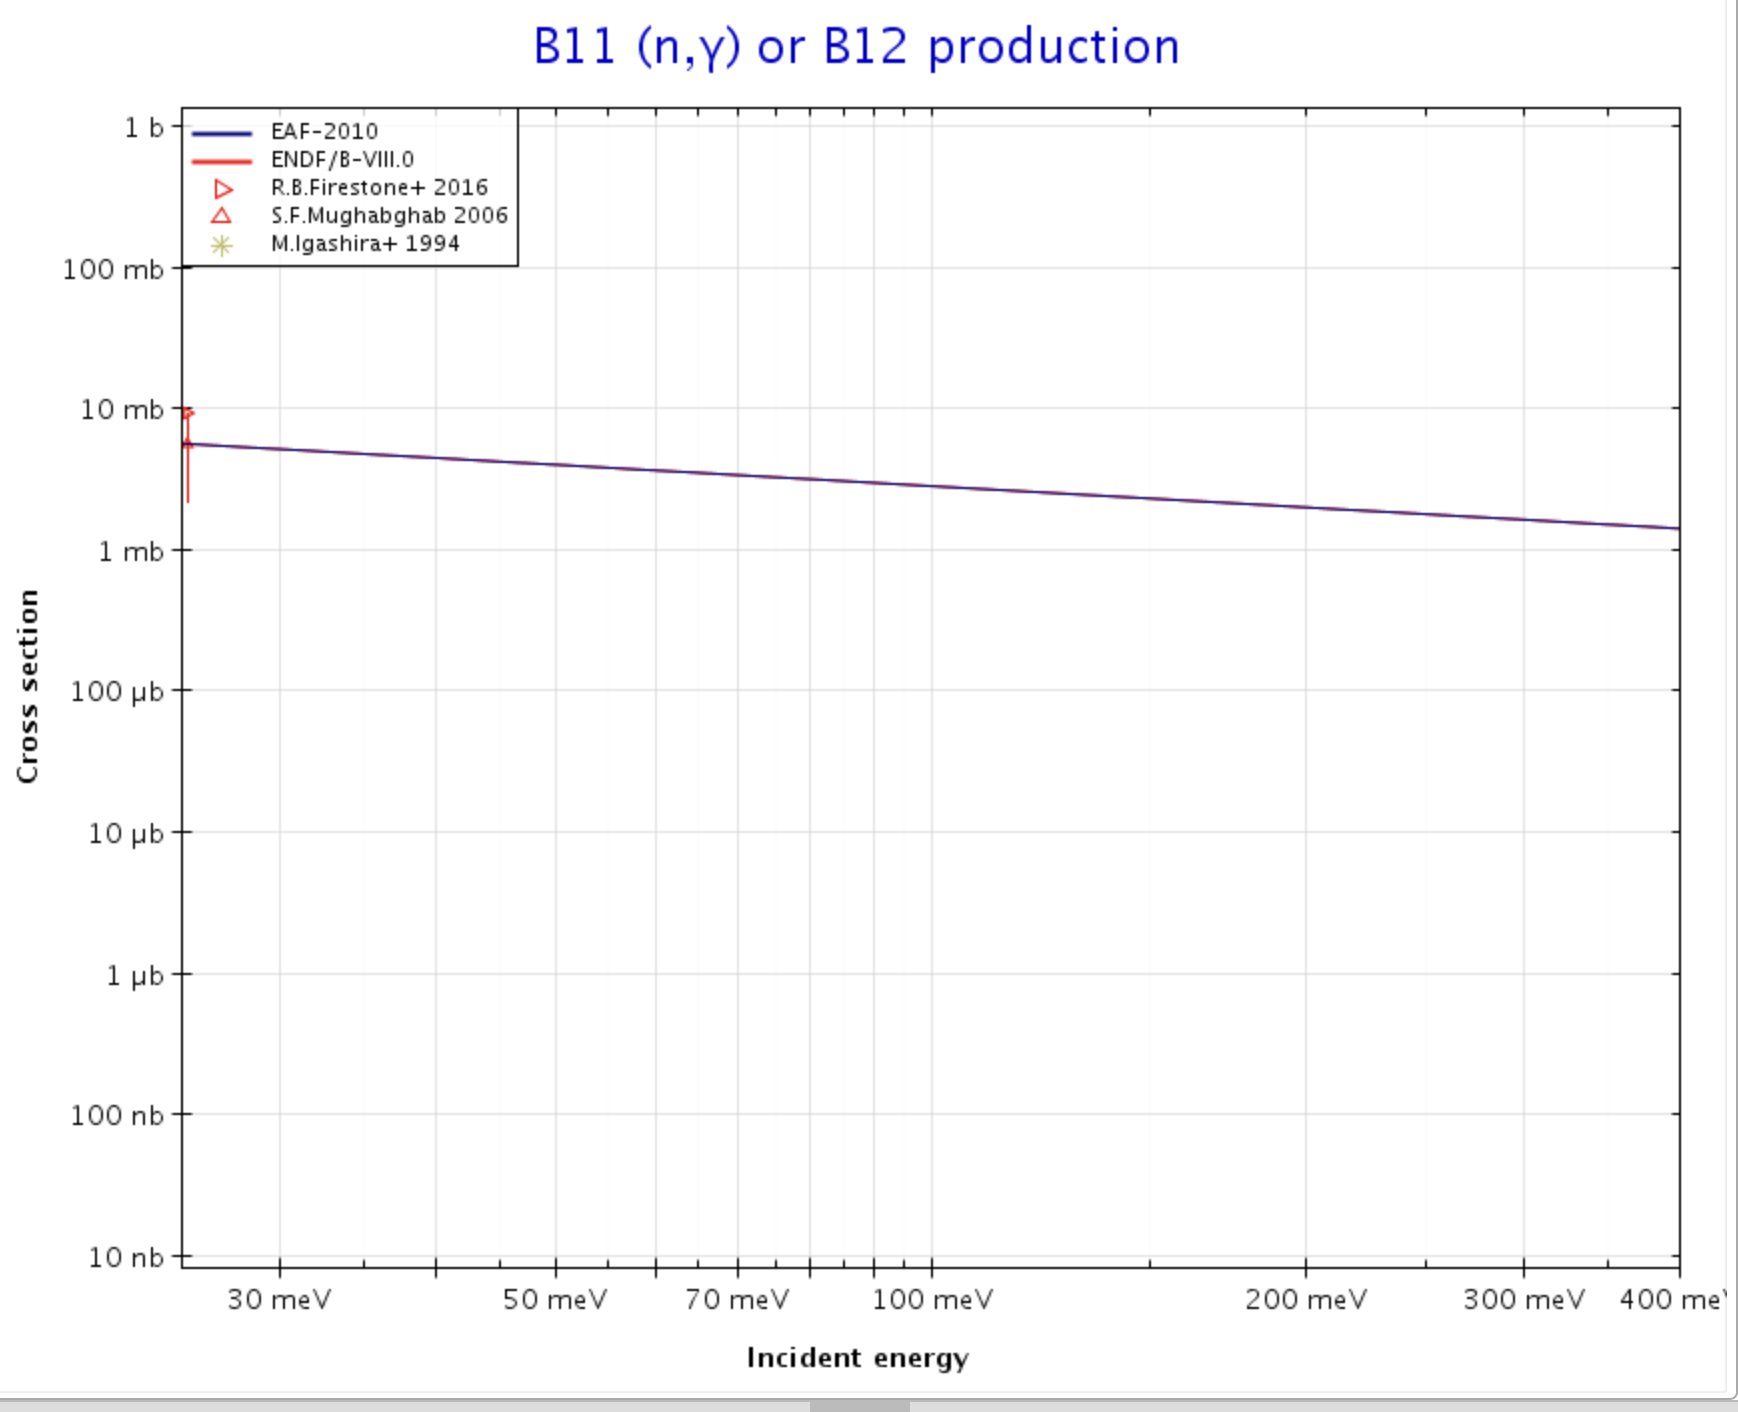
\includegraphics[width = 5.75cm]{Boron-11_Gamma.png}
    \caption{Boron-11 \cite{Kasatov_2016} }
\end{figure}

Neutron poison in fuel like \ce{UB2} can make the Number of neutron in reactor decreaseing and avoid the accident chance, improve the safety margin, and with higher melting temperature, boron can . But in the other hands, neutron poison makes simulation need to think about more circumstance and finally interface the critical operation's problem. But \ce{UB2} more benefits make up for its disadvantage. Please look the next section.

\subsection{Uranium density}

In physicis, density is about a material mass per unit of volume, and larger uranium density which means that the material can contain more uranium atom like U-235, U-233 fissile fuel, it would make longer cycle lengths, and more Uranium atom also means theres have more capture can happened simultaneously.

\begin{table}[ht]
    \caption{The Uranium density campare with \ce{UO2}, recent generation fuel}
    \label{tab:my-table}
    \begin{tabular}{llllll}
    \hline
    The type of ATFs             & \ce{UO2 & UB2  & UN\} & UC   & U3Si2} \\ \hline
    U-Density (U-g/cm$^3$) & 9.6 & 11.7 & 13.5 & 12.7 & 11.3  \\ \hline
    \end{tabular}
\end{table}
\begin{equation}
    \rho = \frac{\Delta k}{k} = \frac{k_{eff}-1}{k_{eff}}
\end{equation} 

Higher Uranium-density will interface the effective neutron multiplication factor like(3), if $k_{eff} = 1$ the system will critical, this result will become a factor in monte-carlo simulation and GEN-IV reactor operation.

\begin{table*}[ht]
    \caption{Thermal conductivity compare with ATFs}
    \label{tab:my-table}
    \begin{tabular}{llllll}
    \hline
    Type of ATFs                                                                      & \ce{UO2          & UB2          & UN            & UC           & U3Si2}         \\ \hline
    \begin{tabular}[c]{@{}l@{}}Thermal conductivity (W/m ·K at 300 °C)\end{tabular} & 6.5(95\% TD) & 25(100\% TD) & 16.6(95\% TD) & 20.4(99\%TD) & 14.7(98\% TD) \\ \hline
    \end{tabular}
    \end{table*}

\subsection{Thermal conductivity}

The thermoldynamics is a huge topic of physicis, but in general, higher thermal conductivity can improved the fuel performance, \ce{UB2} have the best thermal conductivity abillity compare with ATF candidates, such that, the heat can quickly transfer from pellets and coolant according to the heat transfer equation like (4), and \ce{UB2}'s thermal gradient of fuel pellets is smaller than \ce{UO2}, smaller thermal gradient has less thermal stress difference inside, and there is less cracking ( cracking affects heat transfer )

\begin{equation}
    \frac{\partial u}{\partial t} = k \left( \frac{\partial^2 u}{\partial x^2} + \frac{\partial^2 u}{\partial y^2} + \frac{\partial^2 u}{\partial z^2} \right) = k(u_{xx} + u_{yy} + u_{zz})
\end{equation}

This properties is more discuss about fuel economic and safety, occationally, some kind of natural accident like earthquake, tsunami etc. happen, control rods insert into the reactor, the reaction immediately stop and can  make fuel's decay heat more efficiency exchange with coolant, this properties also have benefited on fuel economic, significantly reducing downtime, resulting in increased annual reactor operating time.

\section{Application}
\ce{UB2} talents that make it to be a special role in LWR and next generation reactor, but there have a exception, SMR.

The SMR is brand-new nuclear technology that many country and company are trying to replace the traditional reactor. 

\subsection{Light Water Reactor}
Light Water Reactor have two type, Boling and Pressure( BWR and PWR ), using water(\ce{H2O}) to be the coolant and moderator, \ce{UB2} is design for this originally, with that, the LWR can improve its performance, longer cycle lenghts and reduced stored energy in core, and prevent to occury the accident like Fukushima daiichi nuclear power plant.

\begin{figure}[ht]
    \centering
    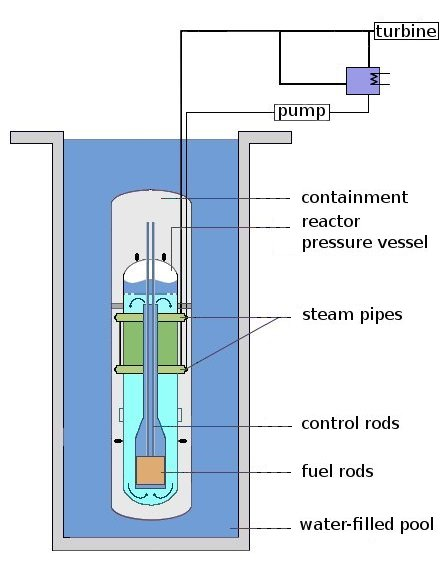
\includegraphics[width = 3.75cm]{Pumpless_light_water_reactor.jpg}
    \caption{The Simple Version of LWR. \cite{wiki:Light-water_reactor} }
\end{figure}

\subsection{Pebble Bed Reactor}
The PBR is a newly reactor design that is suitable for thermal neutron reactor, but if we to change the reflector material and fuel purity of uranium, that will suit for FBR( or other fertile material, the fast neutron breeder reactor is on debating, there's more thing need to developed that finally become a candidate of fast neutron reactor fuel of GEN-IV reactor )

According to \ce{UB2} is ceramic materia, in LWR, we will using metal creamic fuel like \ce{UO2} to make the pellets, but in PBR, the pebble fuel is like TRISO fuel, coated with four layers of three isotropic materials deposited through fluidized chemical vapor deposition \cite{unknown}. 

\ce{UB2} be the contain in TRISO, the coolant like helium can cross the gaps between TRISO, \ce{UB2} high melting temperature can make the counterpart of reator core run at higher temperatures, such the heat transfer equation like (4),and boron can be the safety margin when the PBR function.

\begin{figure}[h]
    \centering
    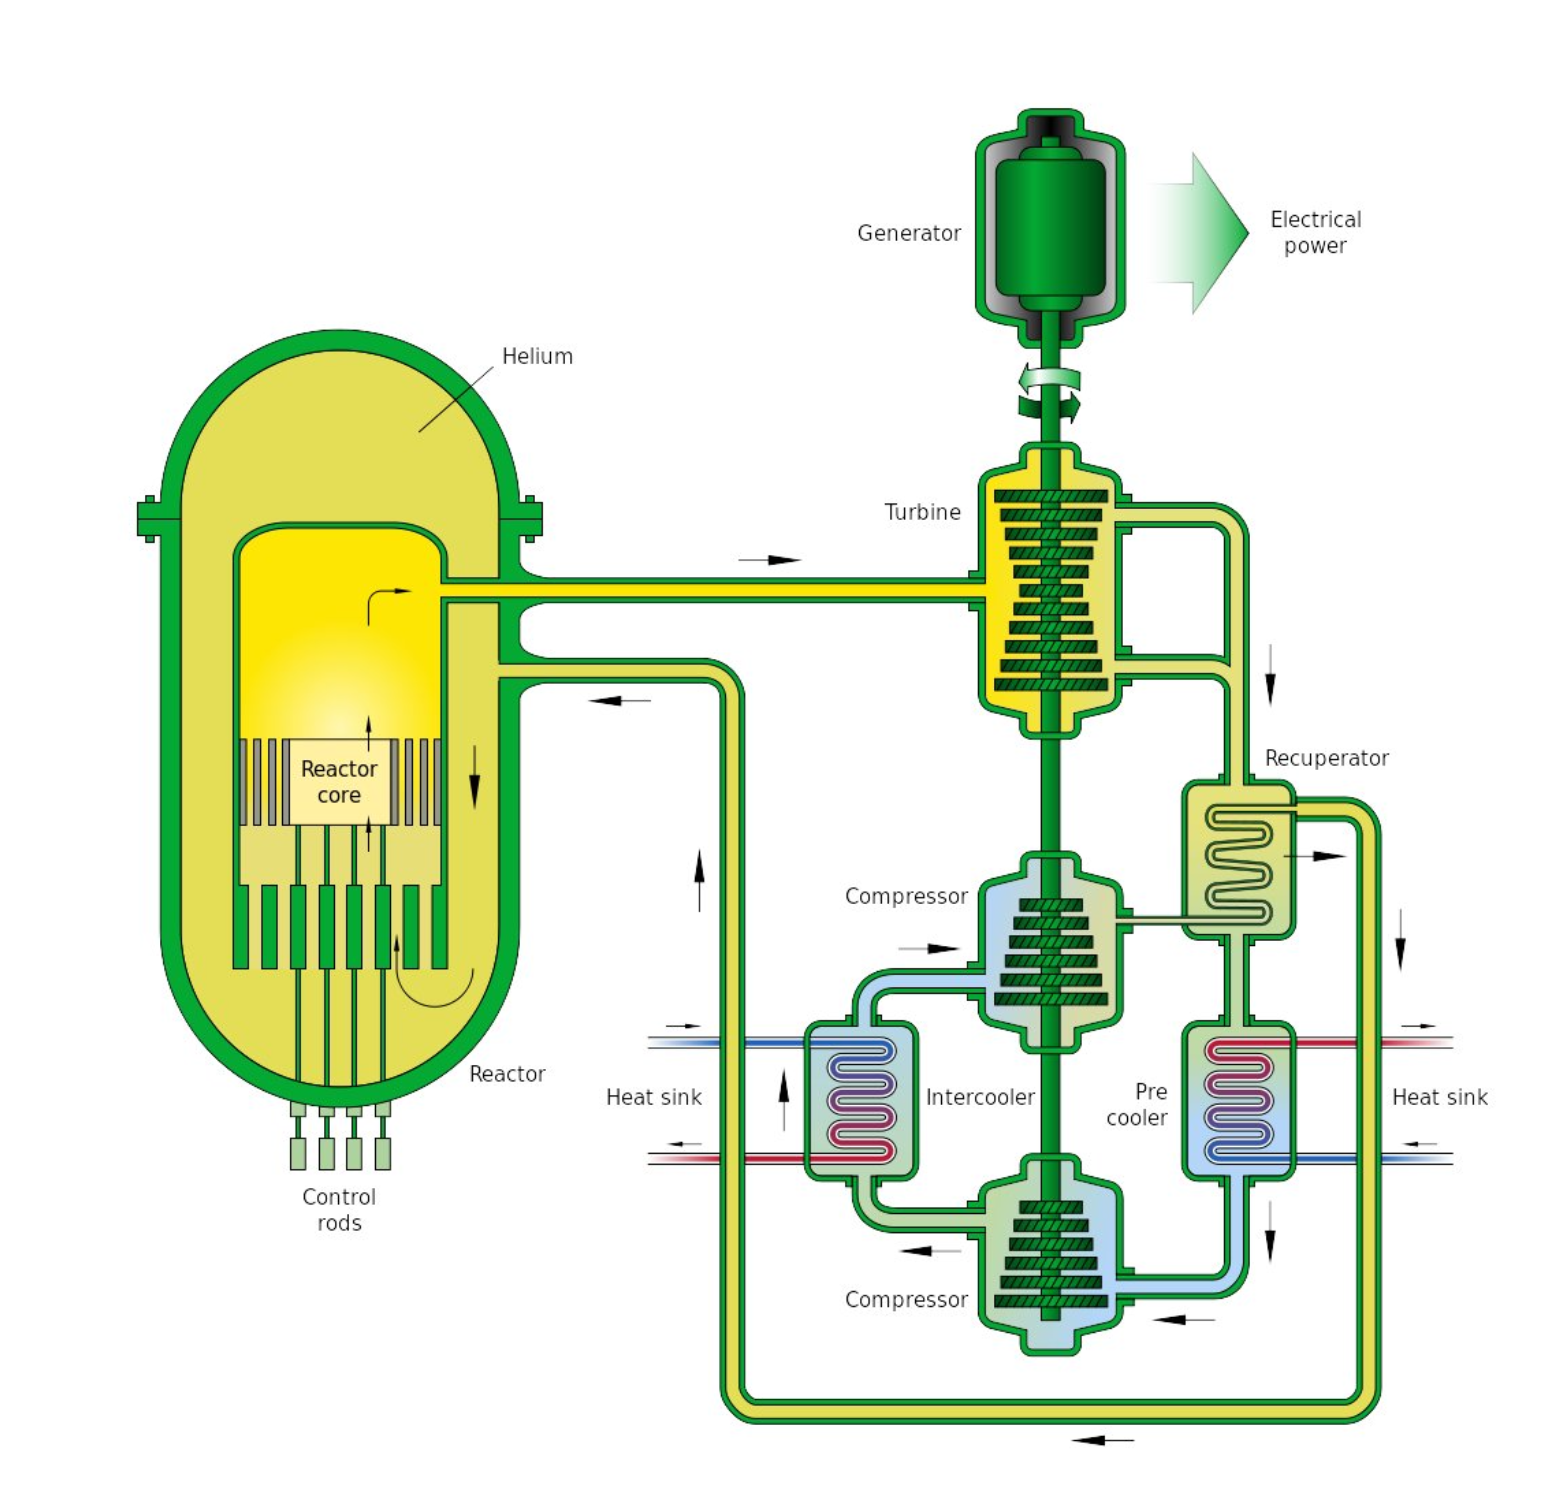
\includegraphics[width = 3.75cm]{gas-cooled.png}
    \caption{The Gas-cooled Fast Reactors \cite{unknown} }
\end{figure}

\subsection{Small Modular Reactor}
SMR is nowadays debating, but almost research is for business running test, the biggest chanllenge of \ce{UB2} is synthesis and enrich the correct purity present of Boron-10 and Boron-11 because burnable neutron poison properties, in a smaller system, the neutron will interface the function as well as \ce{D2O} and \ce{H2O} difference.

But \ce{UB2} is potential candidate fuel with SMR, I hope the day which the \ce{UB2} can supply to factory production line.

\subsection{Nuclear Thearmal Reactor}
This is a special cointerpart with \ce{UB2}, recently, the NASA back to moon project called "Artemis" is planing develope the nuclear technology paving the way for future out of solar explore plans, the nuclear engine and MMR (Micro Modular Reactor, the relative with SMR ) to be the out-space energy supply.

Base on the nuclear is very stable supply source that can afford the mission that is far away of solar system, compare to the traditional energy supply system in spacecraft, the nuclear can using decay heat can via thermoelectric effect to generate the power, this generator early application is on hte Approal Project known as "SNAP-27" or the recnet version of discovery program "ASRG" these reactor is using decay heat to generate the power and heat, but the application in Nuclear Thermal engine need to use the chain-reacton to heat up the fuel like liquid hydrogen.

In traditional chemical rocket engine, the combustion chamber is required combustion accelerant to work, this will decreaseing the containment of fuel, and result in lower specific impulse.

\begin{figure}[h]
    \centering
    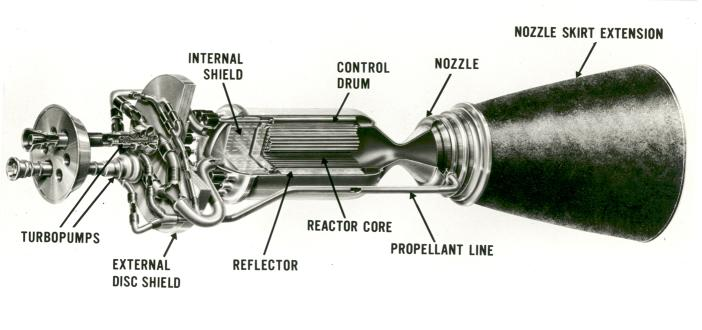
\includegraphics[width = 5.75cm]{NASA-NERVA-diagram.jpg}
    \caption{The early version of NASA VERVA engine design\cite{wiki:Nuclear_thermal_rocket}}
\end{figure}

But with nuclear thermal reactor, the burning chamber is replace chemical with nuclear reactor, the reactor can keep in a stable temperature to heat up the fuel, and don't need the combustion accelerant, this engine will breakthrough the chanllenge in how to design the fuel configuration.

Thermal nuclear rocket is base on phase state to decision the working temperature with the fissle material, gaseous, liquid and solid, in general, the solid have highest working temperature that can make the fuel have maxium performance, but the solid material is very hard to make and its performance is not a big gap with gaseous version, and gaseous is we can make to nuclear thermal rocket.

The \ce{UB2} protential is on developed to be the nuclear thermal rocket fuel material, with that, the explore can (1) more safety due to the safety margin of burnable neutron poison can reduce the chance of accident when the spacecraft on mission (2) Longer specific impulse to significantly increase the disatance of solar explore (3) \ce{UB2} very easy to adminstration, cause its stable physical properties and ceramic hard to crack.

\section{Conclusion}
\ce{UB2} and all of candidate with ATFs, is the most fundamental nuclear technology advanced, with ATFs, the reactor can effect more efficiency and more safety.

In spacecraft, the nuclear generator will become the energy and heat provider when the mission is far from solar system and can explore farther plant with NTR.

Taiwan's goverment need to find a way to solve the energy problem; and the SMR is good methods to using less plant and money to build up a power provide system, Taiwan IC industry is on flourish, and finally the energy problem will grown into a monster.

\bibliographystyle{IEEEtran}
\bibliography{sample}

\end{document}
\endinput
print("meow")
